\documentclass[12pt, a4paper]{article} % General settings in the beginning (defines the document class of your paper)
% 11pt = is the font size
% A4 is the paper size
% “article” is your document class

%----------------------------------------------------------------------------------------
%	Packages
%----------------------------------------------------------------------------------------

% Necessary
\usepackage[german,english]{babel} % English and German language 
\usepackage{booktabs} % Horizontal rules in tables 
% For generating tables, use “LaTeX” online generator (https://www.tablesgenerator.com)
\usepackage{comment} % Necessary to comment several paragraphs at once
\usepackage[utf8]{inputenc} % Required for international characters
\usepackage[T1]{fontenc} % Required for output font encoding for international characters

% Might be helpful
\usepackage{amsmath,amsfonts,amsthm} % Math packages which might be useful for equations
\usepackage{tikz} % For tikz figures (to draw arrow diagrams, see a guide how to use them)
\usepackage{tikz-cd}
\usetikzlibrary{positioning,arrows} % Adding libraries for arrows
\usetikzlibrary{decorations.pathreplacing} % Adding libraries for decorations and paths
\usepackage{tikzsymbols} % For amazing symbols ;) https://mirror.hmc.edu/ctan/graphics/pgf/contrib/tikzsymbols/tikzsymbols.pdf 
\usepackage{blindtext} % To add some blind text in your paper


%---------------------------------------------------------------------------------
% Additional settings
%---------------------------------------------------------------------------------

%---------------------------------------------------------------------------------
% Define your margins
\usepackage{geometry} % Necessary package for defining margins

\geometry{
	top=2cm, % Defines top margin
	bottom=2cm, % Defines bottom margin
	left=2.2cm, % Defines left margin
	right=2.2cm, % Defines right margin
	includehead, % Includes space for a header
	%includefoot, % Includes space for a footer
	%showframe, % Uncomment if you want to show how it looks on the page 
}

\setlength{\parindent}{15pt} % Adjust to set you indent globally 

%---------------------------------------------------------------------------------
% Define your spacing
\usepackage{setspace} % Required for spacing
% Two options:
\linespread{1.5}
%\onehalfspacing % one-half-spacing linespread

%----------------------------------------------------------------------------------------
% Define your fonts
\usepackage[T1]{fontenc} % Output font encoding for international characters
\usepackage[utf8]{inputenc} % Required for inputting international characters

\usepackage{XCharter} % Use the XCharter font


%---------------------------------------------------------------------------------
% Define your headers and footers

\usepackage{fancyhdr} % Package is needed to define header and footer
\pagestyle{fancy} % Allows you to customize the headers and footers

%\renewcommand{\sectionmark}[1]{\markboth{#1}{}} % Removes the section number from the header when \leftmark is used

% Headers
\lhead{} % Define left header
\chead{\textit{}} % Define center header - e.g. add your paper title
\rhead{} % Define right header

% Footers
\lfoot{} % Define left footer
\cfoot{\footnotesize \thepage} % Define center footer
\rfoot{ } % Define right footer

%---------------------------------------------------------------------------------
%	Add information on bibliography
\usepackage{natbib} % Use natbib for citing
\usepackage{har2nat} % Allows to use harvard package with natbib https://mirror.reismil.ch/CTAN/macros/latex/contrib/har2nat/har2nat.pdf

% For citing with natbib, you may want to use this reference sheet: 
% http://merkel.texture.rocks/Latex/natbib.php

%---------------------------------------------------------------------------------
% Add field for signature (Reference: https://tex.stackexchange.com/questions/35942/how-to-create-a-signature-date-page)
\newcommand{\signature}[2][5cm]{%
  \begin{tabular}{@{}p{#1}@{}}
    #2 \\[2\normalbaselineskip] \hrule \\[0pt]
    {\small \textit{Signature}} \\[2\normalbaselineskip] \hrule \\[0pt]
    {\small \textit{Place, Date}}
  \end{tabular}
} % Loads required packages from the separate file 

%---------------------------------------------------------------------------------
%	Define what’s in your document
%---------------------------------------------------------------------------------

\begin{document}

% If you want a cover page, uncomment "%---------------------------------------------------------------------------------
% Cover page
%---------------------------------------------------------------------------------

% Here are more templates for other cover pages: https://www.latextemplates.com/cat/title-pages

% This example is based on this cover page example: https://www.latextemplates.com/template/academic-title-page

\begin{titlepage} % Starts a new environment where the page number is not displayed and the count starts at 1 for the next page

%------------------------------------------------
%	Institutional information
%------------------------------------------------
	
\begin{minipage}{0.4\textwidth} % Begins new environment (like a text box)
    \begin{flushleft} % Sets environment on the left side of the paper
    \large
    University of Bonn\\ % Add your institution
    Research Module in Econometrics and Statistics\\ % Add course title
    \end{flushleft}
\end{minipage}
	
\vspace*{2in} % Adds some space in-between
	
\center % Centre everything on the page

%------------------------------------------------
%	Main part
%------------------------------------------------
	
{\huge\bfseries TITLE OF YOUR PAPER}\\[0.4cm] % Add your paper title 
{\large\today}\\[0.4cm] % Add date (current day)
Lindi Li 3460570 \\
Gewei Cao 3461232 % Add your name
	
\vfill % Adds additional space

%------------------------------------------------
%	General information about the author
%------------------------------------------------


\vfill % Adds additional space

	

	
\end{titlepage}" and comment "\maketitle" as well as "\begin{center} % Center text
    Word count: XXXX
% How to check words in a LaTeX document: https://www.overleaf.com/help/85-is-there-a-way-to-run-a-word-count-that-doesnt-include-latex-commands
\end{center}"


%---------------------------------------------------------------------------------
% Cover page
%---------------------------------------------------------------------------------

% Here are more templates for other cover pages: https://www.latextemplates.com/cat/title-pages

% This example is based on this cover page example: https://www.latextemplates.com/template/academic-title-page

\begin{titlepage} % Starts a new environment where the page number is not displayed and the count starts at 1 for the next page

%------------------------------------------------
%	Institutional information
%------------------------------------------------
	
\begin{minipage}{0.4\textwidth} % Begins new environment (like a text box)
    \begin{flushleft} % Sets environment on the left side of the paper
    \large
    University of Bonn\\ % Add your institution
    Research Module in Econometrics and Statistics\\ % Add course title
    \end{flushleft}
\end{minipage}
	
\vspace*{2in} % Adds some space in-between
	
\center % Centre everything on the page

%------------------------------------------------
%	Main part
%------------------------------------------------
	
{\huge\bfseries TITLE OF YOUR PAPER}\\[0.4cm] % Add your paper title 
{\large\today}\\[0.4cm] % Add date (current day)
Lindi Li 3460570 \\
Gewei Cao 3461232 % Add your name
	
\vfill % Adds additional space

%------------------------------------------------
%	General information about the author
%------------------------------------------------


\vfill % Adds additional space

	

	
\end{titlepage} % Adds a cover page; uncomment if you want a cover page
%\begin{center} % Center text
    Word count: XXXX
% How to check words in a LaTeX document: https://www.overleaf.com/help/85-is-there-a-way-to-run-a-word-count-that-doesnt-include-latex-commands
\end{center} % Gives you the word count; comment if you want a cover page 
%---------------------------------------------------------------------------------
% Table of content
%---------------------------------------------------------------------------------

\newpage % Generates page break

% Table of content
\thispagestyle{empty} % Suppresses page numbers
\tableofcontents % Adds table of content
\newpage % Generates page break

% List of Figures
%\thispagestyle{empty} % Suppresses page numbers
%\listoffigures % Adds list of figures; uncomment if required
%\newpage % Generates page break; uncomment if required

% List of tables
%\thispagestyle{empty} % Suppresses page numbers
%\listoftables % Adds list of tables; uncomment if required
%\newpage % Generates page break; uncomment if required
 % Adds a table of content; uncomment if required

%---------------------------------------------------------------------------------
% Abstract
%---------------------------------------------------------------------------------

\begin{abstract}

\blindtext % Some blind text

\end{abstract} % Adds your abstract
%----------------------------------------------------------------------------------------
% Introduction
%----------------------------------------------------------------------------------------
\setcounter{page}{1} % Sets counter of page to 1

\section{Introduction} % Add a section title
\subsection{Highlighting} % Add a subsection
\LaTeX allows you to highlight text in various ways: \textbf{bold}, \textit{italics}, with \textsc{small caps} or \texttt{as a coding font}.\footnote{ This command adds a footnote to your text.} 

\subsection{Citing} % Add another subsection
Citing in \LaTeX is easy. You could easier cite with the text flow like this ``Referring to.\\
\blindtext % Adds some blintext to your text % Adds your introduction
%----------------------------------------------------------------------------------------
% Literature review
%----------------------------------------------------------------------------------------

\section{Reproducing Kernel Hilbert Space} 

\subsection{Hilbert Space}
The theory of Hilbert space was initiated by David Hilbert. \citet{debnath2005introduction} provides a detailed explanation of Hilbert space $\mathcal{H}$. It is defined as an inner product space that is complete and separable with respect to the norm defined by the inner product.
An example of a defined norm in Hilbert space (i.e, the space $L_2$ of square-integrable functions) can be 
\begin{equation*}
    \parallel f \parallel = \left(\int_a^b f^2(t)dx\right)^\frac{1}{2}.
\end{equation*}
A normed space is a vector space $N$ on which a norm is defined. A non-negative function $\parallel\cdot\parallel$ is a norm if and only if $\forall f,g\in N$ and $\alpha\in\mathbb{R}$:
\begin{itemize}
    \item $\parallel f \parallel \geq 0$ and $\parallel f\parallel=0$ iff $f=0$;
    \item $\parallel f+g \parallel \leq \parallel f \parallel + \parallel g \parallel$;
    \item $\parallel \alpha f\parallel=\mid \alpha \mid \parallel f \parallel$
\end{itemize}
Examples of inner product $<a,b>$ in a Hilbert space are
\begin{itemize}
    \item a usual dot product: $<a,b>=a'b=\sum_i a_i b_i$.
    \item a kernel product: $<a,b>=k(a,b)=\psi(a)'\psi(b)$, where $\psi(a)$ may have infinite dimensions.
\end{itemize} 

\subsection{Introduction to Kernel}
\subsubsection{Feature map}
The motivation of the kernel method is simple. Imagine there are some blue dots and red dots on a vector space $\mathcal{R}^2$ and 
we want to separate them by color. As it is shown in the left-hand side figure, it is difficult to divide them through a straight 
line. However, we may be able to separate them easily by mapping each dot into a high-dimension feature space. The figure below 
shows how the feature map works:
\begin{figure}[htpb!]
    \centering
    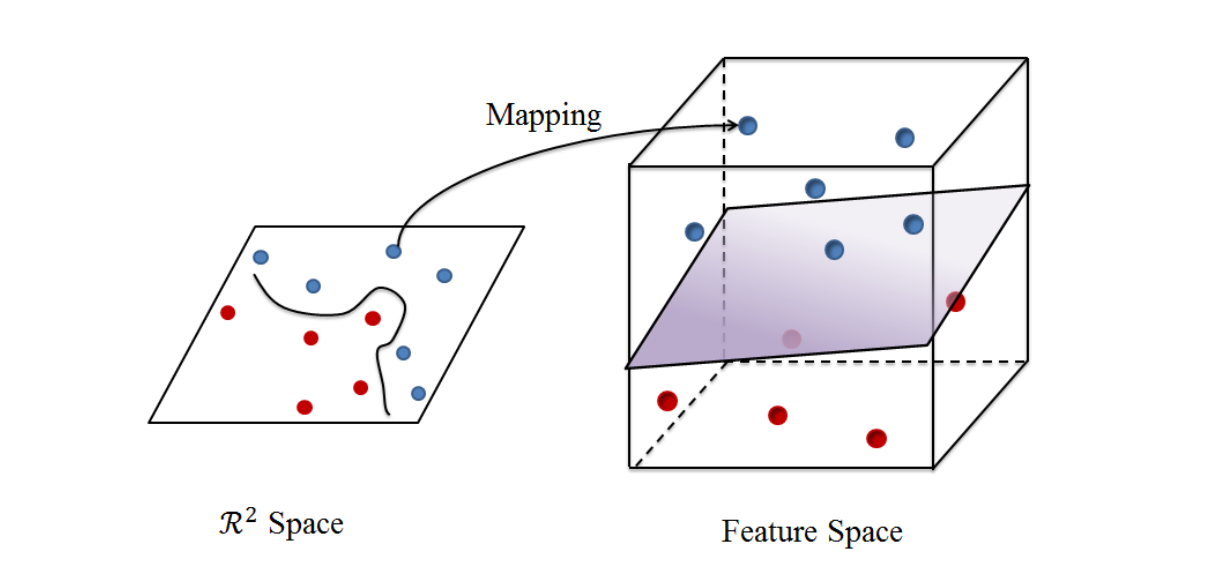
\includegraphics[width=0.7\textwidth]{figure/Mapping.png}
\end{figure}
\\ \\
Let's now use a simple example to illustrate the idea of a feature map. 
we set two vectors $\textbf{x}=\begin{bmatrix}x_1&x_2\end{bmatrix}$ and $\textbf{y}=\begin{bmatrix}y_1&y_2\end{bmatrix}$ in a two-dimension space.
Tow functions $\phi(x)$ and $\phi(y)$ are defined as:
\begin{equation*}
    \phi(x)=\begin{bmatrix}
        x_1x_1&x_1x_2&x_2x_1&x_2x_2
    \end{bmatrix}
\end{equation*}
\begin{equation*}
    \phi(y)=\begin{bmatrix}
        y_1y_1&y_1y_2&y_2y_1&y_2y_2
    \end{bmatrix}
\end{equation*}
We are now successfully mapping them into a four-dimension feature space. 
To write the above example in a general form of linear regression, we first set an equation where $\phi(\cdot)\in\mathcal{R}^m$ and $\phi(x)$ is defined as the mapping function. Note that we assume there is a linear relation between $y$ and $\phi(x)$:
\begin{align}
    y&=\phi(x)^\top w \notag\\
     &= \begin{bmatrix}
        \phi_1(x)\cdots\phi_m(x)
        \end{bmatrix} w
\end{align}
$Y$ and $\Phi$ in generalization is defined by:
\begin{equation}
    Y=\begin{bmatrix}
         y_1&\cdots&y_n
      \end{bmatrix}^\top 
\end{equation}
\begin{align}
    \Phi&=\begin{bmatrix}
           \phi(x_1)&\cdots&\phi(x_n) 
          \end{bmatrix}^\top \notag\\
        &=\begin{bmatrix}
           \phi_1(x_1)&\cdots&\phi_m(x_1)\\
           \vdots&\vdots&\vdots \\
           \phi_1(x_n)&\cdots&\phi_m(x_n)
          \end{bmatrix}
\end{align}
Recall the regularized risk minimization problem of ridge regression. In this case, it can be re-written as:
\begin{align*}
  w{*}&=\underset{w}{\operateorname{argmin}}\sum_{i=1}^n(y_i-\phi(x_i)^\top w)^2+\lambda\parallel w \parallel_2^2 \\
      &=\underset{w}{\operateorname{argmin}}\parallel Y-\Phi w\parallel_2^2+\lambda\parallel w\parallel_2^2
\end{align*}
The least-square solution can also be re-defined by:
\begin{equation}
    w{*}=(\Phi^\top\Phi+\lambda I)^{-1}\Phi^\top Y
\end{equation}
Then we replace $w{*}$ with $(\Phi^\top \Phi+\lambda I)^{-1}\Phi^\top$ in $y=\phi(x)^\top w$, we get:
\begin{align}
    y_w{*} (x)&=\phi(x)^\top w{*}\notag\\
            &=\phi(x)^\top(\Phi^\top \Phi+\lambda I)^{-1}\Phi^\top Y\notag\\
            &=\underbrace{\phi(x)^\top \Phi^\top}_\text{$1\times n$}(\underbrace{\Phi\Phi^\top}_\text{$n\times n$}+\lambda I)^{-1}Y\\
            &\text{using that} (\Phi^\top \Phi+\lambda I)^{-1}\Phi^\top=\Phi^\top(\Phi\Phi^\top+\lambda I)^{-1}\notag
\end{align}


\subsubsection{Kernel Method}
In most cases, it is surprisingly difficult to know and calculate the feature function after mapping. We want to avoid computing $\phi(x)$ in an explicit way, 
especially when $m$ is very large. Therefore, we define a kernel function:
\begin{equation*}
    [\Phi\Phi^\top]_{i,j}=\phi(x_i)^\top \phi(x_j)=K(x_i,x_j)
\end{equation*}
\begin{equation}
    [\phi(x)^\top\Phi^\top]_j=\phi(x)^\top\phi(x_j)=K(x,x_j)
\end{equation}
This is simply the intuition of using the kernel method. For example, the Gaussian kernel is
\begin{equation*}
    k(x_i, x_j) = e^\frac{-\parallel x_i - x_j \parallel}{\sigma^2},
\end{equation*}
Gaussian kernel meaning the similarity between two points where $\parallel x_i - x_j \parallel$ is the Euclidean distance between $x_i$ and $x_j$, and $\sigma^2 \in \mathbb{R}^+$ is the bandwidth of the kernel function. As shown in \citet{hofmann2008kernel}, it has the following properties:\\
for $k: \mathcal{X} \times \mathcal{X} \rightarrow \mathbb{R}$ is a kernel if
\begin{itemize}
    \item $k$ is symmetric: $k(x,y) = k(y,x)$.
    \item $k$ is positive semi-definite, meaning that $\sum_{i} \sum_{j} \alpha_i \alpha_j k(x_i,x_j)\geq0, \forall \alpha_i, \alpha_j \in \mathbb{R}, x \in \mathbb{R}^\mathbb{D}, \mathbb{D} \in \mathbb{Z}^+$. 
    \item We define the corresponding kernel matrix as the matrix $K$ with entries $k_{ij}=k(x_i,x_j)$, the sencond property of $k$ is equivalent to saying that $\textbf{a}'K \textbf{a}\geq 0$.
\end{itemize}
Now we can define a function k: $\mathcal{X} \times \mathcal{X}  \rightarrow \mathbb{R}$ is a kernel if and 
only if there exists a Hilbert space $\mathcal{H}$ and a map $\phi: \mathcal{X}\rightarrow\mathcal{H}$ such that $k(x,y)=\langle\phi(x),\phi(y)\rangle$. \\
Recall the simple example above, instead of computing the inner product of $\langle\phi(x),\phi(y)\rangle$, we can define 
a corresponding kernel function $K(\textbf{x},\textbf{y})=\langle\textbf{x},\textbf{y}\rangle^2$. It can be easily proofed that $K(\textbf{x},\textbf{y})$ is the same as $\langle\phi(\textbf{x}),\phi(\textbf{y})\rangle$:
\begin{align*}
    K(\textbf{x},\textbf{y})&=\langle\textbf{x},\textbf{y}\rangle^2\\
                            &=(x_1y_1+x_2y_2)^2\\
                            &=x_1^2y_1^2+2x_1y_2x_2y_1+x_2^2y_2^2\\
                            &=\langle\phi(\textbf{x}),\phi(\textbf{y})\rangle
\end{align*}

\subsection{Reproducing Kernel Hilbert Space}
Consider a Hilbert space $\mathcal{H}$ full of real-valued functions from $\mathcal{X}$ to $\mathbb{R}$, and a mapping $\Phi: \mathcal{X}\rightarrow\mathbb{R}^\chi$ defined as $x\rightarrow\Phi(x)=k_x=k(\cdot , x)$. A function $k:\mathcal{X}\times\mathcal{X}\rightarrow\mathbb{R}$ is a 
reproducing kernel of $\mathcal{H}$, and $\mathcal{H}$ is a reproducing kernel Hilbert space, if:
\begin{itemize}
    \item $\forall x \in\mathcal{X}$, $k(\cdot, x)\in\mathcal{H}$,
    \item $\forall x \in\mathcal{X}$, $f\in\mathcal{H}$, $\langlef(\cdot),k(\cdot,x)\rangle_\mathcal{H}=f(x)$, which is the reproducing property.
\end{itemize}
To be more intuitive, a Reproducing Kernel Hilbert Space is a Hilbert space $\mathcal{H}$ with a reproducing kernel whose span is dense in $\mathcal{H}$. Equivalently, an RKHS can be defined as a Hilbert space of valid functions with all evaluation functionals bounded and linear. 

\subsection{Representer Theorem}
In the previous section, we have learned that there is always a pair of $(\mathcal{X},k)$ as a Hilbert space or a subset of that space whenever the input domain $\mathcal{X}$ exists. Such a fact means that we are able to study the various data structures in Hilbert spaces. 
In the practical world, however, it is extremely difficult to study many popular kernels since their Hilbert spaces are known to be infinite-dimensional in almost every case. Especially for the purpose of machine learning, we usually prefer to solve an optimization problem in a finite-dimensional space. \\
This is where the representer theorem is useful. It contributes to simplifying the regularized risk-minimization problem by reducing the infinite-dimensional space to a finite-dimensional vector of optimal coefficients and provides provisions for kernels in training data in machine learning.\\
Suppose we are given a nonempty set $\mathcal{X}$, a positive definite real-valued kernel $k$ on $\mathcal{X}\times\mathcal{X}$, a training sample $(x_1,y_1),\dots,(x_m,y_m)\in\mathcal{X}\times\mathbb{R}$, a strictly monotonically increasing real-valued function $f$ on $[0,\infty[$. As explained in \citet{scholkopf2001generalized}, we can find the function $f^{*}$ in the RKHS $\mathcal{H}$ satisfying:
\begin{equation*}
    \mathcal{J}(f^{*})=\underset{f\in\mathcal{H}}{min}\mathcal{J}(f),
\end{equation*}
where 
\begin{equation*}
    \mathcal{J}(f)=L_y(f(x_1),\cdots,f(x_n))+\Omega(\parallel f \parallel_\mathcal{H}^2).
\end{equation*}
Note that $\Omega$ is a non-decreasing regularizer and $y$ is a vector of $y_i$. \\
In the simplest form of machine learning, in order to predict $x$, the algorithm collects the samples in the training set $\mathcal{X}$ that are similar to $x$, 
and then takes the weighted value of these samples as the predict value of $x$. Here comes the questions:
\begin{itemize}
    \item How to measure the similarity between samples?
    \item How to weigh the value of each sample?
\end{itemize} 
In general, the higher the similarity of the sample to our point of interest $x$, the more the sampling weights. To evaluate the similarity between two observations, 
a kernel is defined as a function of two input patterns $k(x_i, x_j)$, mapping onto a real-valued output. \citet{hofmann2008kernel} wrote that the advantage of using such a kernel as a similarity measure is that it allows us to construct algorithms in dot product spaces.\\
The representer theorem is that the solution to $\underset{f\in\mathcal{H}}{min}[L_y(f(x_1),\cdots,f(x_n))+\Omega(\parallel f \parallel_\mathcal{H}^2)]$ can 
be written in a simpler version, which takes the form $f^{*}=\sum_{i=1}^n\alpha_i k(x_i,\cdot)$, where $\alpha_i$ the weighted value of each sample and $k$ is the similarity measure. If $\Omega$ is strictly increasing, all solutions apply to this form. 


\subsection{Example Using Representer Theorem--Kernel Ridge Regression}
Suppose we are given empirical data $(y_1,x_1),\dots,(y_n,x_n)$, where $i = 1, \dots, N$. Assume $y=g(x)$ in RKHS. We want to estimate the function $g(\cdot)$ to minimize
\begin{equation}
    \underset{g\in\mathcal{H}}{min}\sum_{i=1}^N(y_i-g(x_i))^2+\Omega\parallel g\parallel_\mathcal{H}^2
\end{equation}
In order to avoid extremely high variance, we impose an additional assumption 
that a smoother curve with fewer oscillations is preferred. We utilize regularization to simplify the function and satisfy the additional assumption by adding a penalty term $\Omega$. Luckily, the representer theorem already tells us that the least squared problem always has a solution of the form 
\begin{equation}
    g(\cdot)^{*}=\sum_{i=1}^N\alpha_i k(\cdot,x_i),
\end{equation}
and according to reproducing property of RKHS, we have
\begin{equation}
    g(x)=\langle g(\cdot), k(\cdot, x)\rangle_\mathcal{H}.
\end{equation}
Also, it is obvious that
\begin{equation}
    \parallel g \parallel^2=\langle g(\cdot),g(\cdot)\rangle.
\end{equation}
We then substitute $(9)$, $(10)$ for $(7)$,
\begin{equation*}
    \underset{g\in\mathcal{H}}{min}\sum_{i=1}^N(y_i-\langle g(\cdot),k(\cdot, x)\rangle)^2+\Omega\langle g(\cdot),g(\cdot)\rangle,
\end{equation*}
and plug $(8)$ in $(7)$ and get
\begin{equation*}
    \underset{\alpha}{min}\sum_{i=1}^N(y_i-\langle \sum_{j=1}^N\alpha_j k(\cdot, x_j),k(\cdot,x_i)\rangle)^2+\Omega\langle \sum_{i=1}^N\alpha_i k(\cdot, x_i),k(\cdot,x_j)\rangle\\
\end{equation*}
\begin{equation*}
    \Rightarrow\underset{\alpha}{min}\sum_{i=1}^N(y_i-\sum_{j=1}^N\alpha_j k(x_j,x_i))^2+\Omega\sum_{i=j}^N\sum_{i=1}^N\alpha_j\alpha_i k(x_i,x_j)
\end{equation*}
Remember the corresponding kernel matrix as the matrix $K$ with entries $k_{ij}=k(x_i,x_j)$ is equivalent to saying that $\textbf{a}'K \textbf{a}\geq 0$, we can then rewrite the kernel ridge regression as:
\begin{equation*}
    \parallel y_i-K \textbf{a}\parallel^2+\Omega \textbf{a}' K\textbf{a}.
\end{equation*}
By differentiation and setting the equation $(9)$ to zero, we get:
\begin{equation}
    \alpha^{*}=(K+\Omega I_n)^{-1}y.
\end{equation}


\subsection{Example of Solving the Kernel Function}
In this paper, we study in the RKHS $\mathcal{H} = \mathcal{H}_{\omega ,\delta}$ consisting of differentiable functions $ h : [0, \infty ) \to \mathbb{R}$ of the form $h(x) = \int_{0}^{x} h'(t) dt$ with continuous derivatives, $h'(x) = h'(0) + \int_{0}^{x} h''(t)dt $ for integrable $h''$, and with finite norm 
\begin{equation}
\langle h, h\rangle = \parallel h \parallel_{\omega ,\delta} = (\int_{0}^{\infty} (\delta h'(x)^2 + (1 - \delta)h''(x)^2)\omega (x)dx)^{\frac{1}{2}}
\end{equation}
for some measurable weight function $\omega : [0, \infty) \to [1, \infty)$ and shape parameter $\delta \in (0,1)$. With additional assumption in the research paper's appendix A.2, we can extend it to the case $\delta \in \{ 0, 1\}$. \\
The Lemma 3 assumes that for any fixed $y \ge 0$, exists a solution $\phi$ of the linear differential equation 
\begin{equation}
\delta \phi \omega - (1-\delta )(\phi ' \omega)' = 1_{[0,y]}
\end{equation}
and for $\psi  \in \mathcal{H}_{\omega, \delta}, \psi (x) = \int_{0}^{x} \phi (t)dt$, then for $h \in \mathcal{H}_{\omega, \delta}$ with $h'(x) = 0$ for $x > n$ for some finite $n$, we can write 
\begin{equation}
\langle \psi , h\rangle_{\omega, \delta} = \int_{0}^{\infty} (\delta \psi '(x) h'(x) + (1-\delta )\psi '' h''(x))\omega (x)dx
\end{equation}
according to the definition for any $h \in \mathcal{H}_{\omega,\delta}$. The assumption of sloution exists and Lemma 4 could give us that $\langle \psi , h\rangle = h(y)$ which implies that $k(\cdot , y) = \psi$ by the reproducing property. Then  $k(x , y) = \psi (x)$, and remind that $\psi (x) = \int_{0}^{x} \phi (t)dt$, then we can find the form of $k(x,y)$ if we know the form of $\phi$, and we could solve $\phi$ by giving different value of $\delta$ and $\omega$. Below is an example of how to solve the research paper's equation 8. \\
In the research paper, the weight function $\omega (x) = e^{\alpha x}$, if $\alpha = 0, \delta = 1$, then $ \phi = 1_{[0,y]}$, and $k(x,y) = \psi (x) = \int_{0}^{x} 1_{[0,y]} dt = min\{x, y\}$. 
 % Adds your literature review


\section{Gaussian Process and Bayesian Perspective}
After estimating the discount function $g(\boldsymbol{x})$, we want to do inference with this function, and because of the nonparametric estimation, we cannot calculate the statistical distribution of parameters, hence here we use Gaussian Process to estimate the distribution of discount function and construct a confidence interval. 
\subsection{Definition}
We have data $\textbf{D} = \{ (\boldsymbol{x_i}, y_i) \} _{i=1} ^{M}$, and assume that mean of y is 0. 
\\ \\
Task: find the distribution of $ f^{*}(x) $.  
\\ \\
Assume that the true form of prediction function is: $y_i = f(\boldsymbol{x_i}) + \epsilon_i$ and $\epsilon_i \sim \mathcal{N}(0,\sigma_{i}^{2})$. Here we have an M dimensional dependent variable \textbf{y}, and a $M \times N$ dimensional independent variable \textbf{X}, where M is the number of observations, and N is the dimension of x, i.e. $\boldsymbol{x_i}\in \mathbb{R}^N $. The function 
$f(\boldsymbol{x_i}) : \mathbb{R}^N \to \mathbb{R}$ takes vector $\boldsymbol{x_i} \in \mathbb{R}^N$. Let $\boldsymbol{K}_{X, X} = k(\boldsymbol{x},\boldsymbol{x}^T)$ which is the matrix of $k(\boldsymbol{x_i}, \boldsymbol{x_j})$. Thus, \textbf{K} is a $M \times M$ matrix. 
\\ \\
The assumption of the Gaussian Process is as follows: \\ \\
For a given vector \textbf{y}, and its corresponding data \textbf{X}, where vector $ \boldsymbol{y} \in \mathbb{R}^M$ and $\boldsymbol{X}$ is $M \times N$ matrix. In addition, for \textbf{y} and \textbf{X} data, the error term $\epsilon \sim \mathcal{N}(\boldsymbol{0},\varSigma^{\epsilon})$, and $\varSigma^{\epsilon} = diag(\sigma_{1}^{2}, \sigma_{2}^{2}, \sigma_{3}^{2}, ......, \sigma_{M}^{2}) $.  Meanwhile we have arbitrary $n \times N$ matrix \textbf{Z} and predicted value $f^{*}(\boldsymbol{z}) \in \mathbb{R}^n$, where $ \boldsymbol{z} = (\boldsymbol{z_1, z_2, z_3, ......, z_n})^T$. \\ \\
Then we assume \textbf{y} and $f^{*}(\boldsymbol{z})$ follow a $(M + n)$ multivariate normal distribution(MVN): \\
\begin{equation}
\begin{bmatrix}
f^{*}(\boldsymbol{z}) \\
\boldsymbol{y} 
\end{bmatrix} \sim \mathcal{N}
\begin{pmatrix}
\begin{bmatrix}
\mu_{f^{*}(\boldsymbol{z})} \\ \mu_{\boldsymbol{y}}
\end{bmatrix} 
 & ,\begin{bmatrix}
\boldsymbol{K}_{Z, Z} & \boldsymbol{K}_{Z, X} \\
\boldsymbol{K}_{X, Z} & \hat{\boldsymbol{K}}_{X, X}
\end{bmatrix}
\end{pmatrix}
\end{equation}
where $ \hat{\boldsymbol{K}}_{X, X} = \boldsymbol{K}_{X, X} + \varSigma^{\epsilon}$. \\ \\
Then given data \textbf{y}, \textbf{X} and \textbf{Z}, according to the conditional distributions of the multivariate normal distribution\footnote{https://statproofbook.github.io/P/mvn-cond}, we have the posterior distribution 
\begin{equation}
 f^{*}(\boldsymbol{z}) | \boldsymbol{y}, \boldsymbol{X},  \boldsymbol{Z} \sim  \mathcal{N}(\mu_{f^{*}(\boldsymbol{z})} + \boldsymbol{K}_{Z, X}\hat{\boldsymbol{K}}_{X, X}^{-1}(\boldsymbol{y} - \mu_{\boldsymbol{y}}), \boldsymbol{K}_{Z, Z} - \boldsymbol{K}_{Z, X}\hat{\boldsymbol{K}}_{X, X}^{-1}\boldsymbol{K}_{X, Z})
\end{equation}

\subsection{Intuition behind Gaussian Process}
The idea behind this process is that, assume our interested function is $f(x)$, $ f(\boldsymbol{x}): \mathbb{R}^N \to \mathbb{R}$, and we have an arbitrary vector of independent variable $\boldsymbol{x} = (\boldsymbol{x_1}, \boldsymbol{x_2,} ......, \boldsymbol{x_M})^T$, and for each $\boldsymbol{x_i}, i = 1, 2, ...,M, x_i \in \mathbb{R}^N$, then we can obtain a series of $f(\boldsymbol{x})= (f(\boldsymbol{x_1}), f(\boldsymbol{x_2}), f(\boldsymbol{x_3}), ......, f(\boldsymbol{x_M}) )^T$. We assume that the series of f(\textbf{x}) follows a multivariate normal distribution which is: 

\begin{equation}
f(\boldsymbol{x}) \sim \mathcal{N}(\mu(\boldsymbol{x}), k(\boldsymbol{x},\boldsymbol{x}^T)) 
\end{equation}
\\ 
This is the prior distribution of our function $f(x)$, here we have a set of infinite functions that follow this distribution, their mean is the function $\mu(\boldsymbol{x_i})$, and the variance of them is $k(\boldsymbol{x_i},\boldsymbol{x_i}^T)$. This makes the distribution of $f(\boldsymbol{x})$ to be called Gaussian Process (GP). Note that if we add a noise term $\epsilon \sim \mathcal{N}(\boldsymbol{0},\varSigma^{\epsilon})$, then our prior distribution of $y = f(\boldsymbol{x}) + \epsilon \sim \mathcal{N}(\mu(\boldsymbol{x}), k(\boldsymbol{x},\boldsymbol{x}^T) + \varSigma^{\epsilon})$ is also a Gaussian Process. Here we use the kernel matrix to denote the variance-covariance matrix because the kernel value represents how near two data points in the space are, with this property we can obtain a smooth function.  \\ \\
Remind that our goal is to estimate the distribution of $f(\boldsymbol{x^*})$ given observed training data set $D = \{\boldsymbol{x_i}, y_i\}_{i = 1}^M$ and test data set $\{\boldsymbol{x_j^*}\}_{j = 1}^n$. Firstly we compare our nonparametric case to a parametric case. In a parametric case, assume the parameter $\theta$ determines the form of $f_{\theta}(\cdot)$, according to the Bayesian rule, 
$
p(\boldsymbol{y^*} | \boldsymbol{x^*}, \boldsymbol{x}, \boldsymbol{y}) = \int_{\theta} p(\boldsymbol{y^*}, \theta |  \boldsymbol{x^*}, \boldsymbol{x}, \boldsymbol{y})d\theta = \int_{\theta} p(\boldsymbol{y^*} | \theta, \boldsymbol{x^*})p(\theta | \boldsymbol{x}, \boldsymbol{y})d\theta
$
, where $\boldsymbol{y^*}$ is the prediction of given data $\boldsymbol{x^*}$, and its form of model is determmined by paramater $\theta$. The estimated $\theta$ value is determined by training data $D$. This is to say that we update our parameter $\theta$ by given $D$, and use $p(\theta |  \boldsymbol{x}, \boldsymbol{y})$ as a new prior probability, and based on this to predict posterior of $\boldsymbol{y^*}$.  \\ \\
Therefore, back to our GP nonparametric case, $\theta$ could be substituted by function $f(\cdot)$. One can show that the joint distribution of $(f(\boldsymbol{x^*}), \boldsymbol{y})^T$ follows a multivariate normal distribution as in the definition before, because of the assumption of GP and the property of MVN. With the joint distribution, we want to find posterior probability:  $p(f(\boldsymbol{x^*}) | \boldsymbol{x^*}, \boldsymbol{x}, \boldsymbol{y}) = \int p(f(\boldsymbol{x^*})  | f, \boldsymbol{x^*})p(f | \boldsymbol{x}, \boldsymbol{y})df$, where $p(f | \boldsymbol{x}, \boldsymbol{y})$ is the posterior of $f(\cdot)$ given $D$, and is regarded as prior when estimating $p(f(\boldsymbol{x^*}) | \boldsymbol{x^*}, D)$, this process is called Bayesian updating. Fortunately, we do not need to take any integral in GP, because the posterior of $f(\boldsymbol{x^*})$ could be calculated by the formula of conditional distribution in MVN as mentioned in the former section. 

\subsection{Gaussian Process in research paper}
In this research paper, authors assumed discount function $g(\boldsymbol{z})$ given a vector of different maturties $\boldsymbol{z} = (z_1, z_2, ......, z_n)$ follows a MVN distribution $\mathcal{N}(m(\boldsymbol{z}), k(\boldsymbol{z}, \boldsymbol{z}^T))$. Then this is a Gaussian Process, and by Bayesian updating for given price $P$, corresponding cash flow matrix $C$, and time to maturities $x$, we can obtain the posterior mean and variance function in the research paper's equation (12) and equation (13). Therefore, the variance function of MVN could give us the confidence interval of $g(z)$ i.e. for each maturity time $z$ we calculate $k^{post}(z,z)$ as its normal variance, which could help us to evaluate the precision of our prediction. Furthermore, with the posterior distribution of $g(\boldsymbol{x})$, it is implied that the coupon bond price $Cg(\boldsymbol{x}) \sim \mathcal{N}(Cm^{post}(\boldsymbol{x}), Ck^{post}(\boldsymbol{x},\boldsymbol{x}^T)C^T)$. \\ \\
Note that authors assume the variance covariance matrix of error term $\varSigma^{\epsilon} = diag(\sigma_{1}^{2}, \sigma_{2}^{2}, \sigma_{3}^{2}, ......, \sigma_{M}^{2}) $ where diagnoal elements all satisify $\omega_i = \frac{\lambda}{\sigma_{i}^{2}}$, this implies that we give a higher weight for a bond price which has less noise. In addition, we assume that the prior mean function is constant $m(x) = 1$ which assumes no time value of money. With these assumptions, the posterior mean function coincides with estimated $\hat{g}(\boldsymbol{x})$ as in the research paper's equation (5). 



 % Adds your theory section 
%----------------------------------------------------------------------------------------
% Research design
%----------------------------------------------------------------------------------------

\section{Research Design}

\blindtext % Some blind text
 % Adds your research design
%%----------------------------------------------------------------------------------------
% Analysis
%----------------------------------------------------------------------------------------

\section{Analysis}

\blindtext % Some blind text % Adds your analysis
%----------------------------------------------------------------------------------------
% Conclusion
%----------------------------------------------------------------------------------------

\section{Conclusion}

\blindtext % Some blind text
 % Adds your conclusion
%----------------------------------------------------------------------------------------
% Bibliography
%----------------------------------------------------------------------------------------
\newpage % Includes a new page

\pagenumbering{roman} % Changes page numbering to roman page numbers
%\bibliography{literature}

\bibliography{literature.bib} % Add the filename of your bibliography
\bibliographystyle{apsr} % Defines your bibliography style

% For citing, please see this sheet: http://merkel.texture.rocks/Latex/natbib.php % Adds your references
%----------------------------------------------------------------------------------------
% Appendix
%----------------------------------------------------------------------------------------
\newpage % Includes a new page
\section*{Appendix} % Stars disable section numbers
% \appendix % Uncomment if you want to add an "automatic" appendix
\pagenumbering{Roman} % Changes page numbering to Roman page numbers

\blindtext % Adds some blind text% Adds an appendix
%%----------------------------------------------------------------------------------------
% Declaration
%----------------------------------------------------------------------------------------
\newpage % Includes a page break
\thispagestyle{empty} % Leaves the page style empty (no page number, no header, no footer)
\section*{Statutory Declaration} % Stars disable section numbers

\begin{otherlanguage}{german}
Hiermit versichere ich, dass diese Arbeit von mir pers\"{o}nlich verfasst ist und dass ich keinerlei fremde Hilfe in Anspruch genommen habe. Ebenso versichere ich, dass diese Arbeit oder Teile daraus weder von mir selbst noch von anderen als Leistungsnachweise andernorts eingereicht wurden. W\"{o}rtliche oder sinngem\"{a}{\ss}e \"{U}bernahmen aus anderen Schriften und Ver\"{o}ffentlichungen in gedruckter oder elektronischer Form sind gekennzeichnet. S\"{a}mtliche Sekund\"{a}rliteratur und sonstige Quellen sind nachgewiesen und in der Bibliographie aufgef\"{u}hrt. Das Gleiche gilt f\"{u}r graphische Darstellungen und Bilder sowie f\"{u}r alle Internet-Quellen. Ich bin ferner damit einverstanden, dass meine Arbeit zum Zwecke eines Plagiatsabgleichs in elektronischer Form anonymisiert versendet und gespeichert werden kann. Mir ist bekannt, dass von der Korrektur der Arbeit abgesehen und die Pr\"{u}fungsleistung mit nicht ausreichend bewertet werden kann, wenn die Erkl\"{a}rung nicht erteilt wird.
\end{otherlanguage}

\vspace*{1in} % Adds extra space between two paragraphs

\noindent I hereby declare that the paper presented is my own work and that I have not called upon the help of a third party. In addition, I affirm that neither I nor anybody else has submitted this paper or parts of it to obtain credits elsewhere before. I have clearly marked and acknowledged all quotations or references that have been taken from the works of others. All secondary literature and other sources are marked and listed in the bibliography. The same applies to all charts, diagrams and illustrations as well as to all Internet resources. Moreover, I consent to my paper being electronically stored and sent anonymously in order to be checked for plagiarism. I am aware that the paper cannot be evaluated and may be graded ``failed'' (``nicht ausreichend'') if the declaration is not made.\\

%\vspace*{1in} % Adds extra space

% Add field for signature, date, and place
\hfill \signature{} 
 % Adds your declaration


%---------------------------------------------------------------------------------

\end{document}
